%% bare_conf.tex
%% V1.4b
%% 2015/08/26
%% by Michael Shell
%% See:
%% http://www.michaelshell.org/
%% for current contact information.
%%
%% This is a skeleton file demonstrating the use of IEEEtran.cls
%% (requires IEEEtran.cls version 1.8b or later) with an IEEE
%% conference paper.
%%
%% Support sites:
%% http://www.michaelshell.org/tex/ieeetran/
%% http://www.ctan.org/pkg/ieeetran
%% and
%% http://www.ieee.org/

%%*************************************************************************
%% Legal Notice:
%% This code is offered as-is without any warranty either expressed or
%% implied; without even the implied warranty of MERCHANTABILITY or
%% FITNESS FOR A PARTICULAR PURPOSE! 
%% User assumes all risk.
%% In no event shall the IEEE or any contributor to this code be liable for
%% any damages or losses, including, but not limited to, incidental,
%% consequential, or any other damages, resulting from the use or misuse
%% of any information contained here.
%%
%% All comments are the opinions of their respective authors and are not
%% necessarily endorsed by the IEEE.
%%
%% This work is distributed under the LaTeX Project Public License (LPPL)
%% ( http://www.latex-project.org/ ) version 1.3, and may be freely used,
%% distributed and modified. A copy of the LPPL, version 1.3, is included
%% in the base LaTeX documentation of all distributions of LaTeX released
%% 2003/12/01 or later.
%% Retain all contribution notices and credits.
%% ** Modified files should be clearly indicated as such, including  **
%% ** renaming them and changing author support contact information. **
%%*************************************************************************


% *** Authors should verify (and, if needed, correct) their LaTeX system  ***
% *** with the testflow diagnostic prior to trusting their LaTeX platform ***
% *** with production work. The IEEE's font choices and paper sizes can   ***
% *** trigger bugs that do not appear when using other class files.       ***                          ***
% The testflow support page is at:
% http://www.michaelshell.org/tex/testflow/



\documentclass[conference]{IEEEtran}
% Some Computer Society conferences also require the compsoc mode option,
% but others use the standard conference format.
%
% If IEEEtran.cls has not been installed into the LaTeX system files,
% manually specify the path to it like:
% \documentclass[conference]{../sty/IEEEtran}





% Some very useful LaTeX packages include:
% (uncomment the ones you want to load)


% *** MISC UTILITY PACKAGES ***
%
%\usepackage{ifpdf}
% Heiko Oberdiek's ifpdf.sty is very useful if you need conditional
% compilation based on whether the output is pdf or dvi.
% usage:
% \ifpdf
%   % pdf code
% \else
%   % dvi code
% \fi
% The latest version of ifpdf.sty can be obtained from:
% http://www.ctan.org/pkg/ifpdf
% Also, note that IEEEtran.cls V1.7 and later provides a builtin
% \ifCLASSINFOpdf conditional that works the same way.
% When switching from latex to pdflatex and vice-versa, the compiler may
% have to be run twice to clear warning/error messages.






% *** CITATION PACKAGES ***
%
\usepackage{cite}
% cite.sty was written by Donald Arseneau
% V1.6 and later of IEEEtran pre-defines the format of the cite.sty package
% \cite{} output to follow that of the IEEE. Loading the cite package will
% result in citation numbers being automatically sorted and properly
% "compressed/ranged". e.g., [1], [9], [2], [7], [5], [6] without using
% cite.sty will become [1], [2], [5]--[7], [9] using cite.sty. cite.sty's
% \cite will automatically add leading space, if needed. Use cite.sty's
% noadjust option (cite.sty V3.8 and later) if you want to turn this off
% such as if a citation ever needs to be enclosed in parenthesis.
% cite.sty is already installed on most LaTeX systems. Be sure and use
% version 5.0 (2009-03-20) and later if using hyperref.sty.
% The latest version can be obtained at:
% http://www.ctan.org/pkg/cite
% The documentation is contained in the cite.sty file itself.






% *** GRAPHICS RELATED PACKAGES ***
%
\ifCLASSINFOpdf
  \usepackage[pdftex]{graphicx}
  % declare the path(s) where your graphic files are
  % \graphicspath{{../pdf/}{../jpeg/}}
  % and their extensions so you won't have to specify these with
  % every instance of \includegraphics
  % \DeclareGraphicsExtensions{.pdf,.jpeg,.png}
\else
  % or other class option (dvipsone, dvipdf, if not using dvips). graphicx
  % will default to the driver specified in the system graphics.cfg if no
  % driver is specified.
  % \usepackage[dvips]{graphicx}
  % declare the path(s) where your graphic files are
  % \graphicspath{{../eps/}}
  % and their extensions so you won't have to specify these with
  % every instance of \includegraphics
  % \DeclareGraphicsExtensions{.eps}
\fi


\usepackage{graphicx}
\usepackage{float}
\usepackage{booktabs}
\usepackage[table,xcdraw]{xcolor}
\usepackage{tabularx}
\usepackage[table]{xcolor}

\definecolor{lightGrey}{RGB}{240,240,240}

% correct bad hyphenation here
\hyphenation{op-tical net-works semi-conduc-tor}


\begin{document}
%
% paper title
% Titles are generally capitalized except for words such as a, an, and, as,
% at, but, by, for, in, nor, of, on, or, the, to and up, which are usually
% not capitalized unless they are the first or last word of the title.
% Linebreaks \\ can be used within to get better formatting as desired.
% Do not put math or special symbols in the title.
\title{Introducing Virtual Reality \\ in Robot Assisted Minimally Invasive \\ Surgery Team Training}


% author names and affiliations
% use a multiple column layout for up to three different
% affiliations
%\author{\IEEEauthorblockN{Michael Shell}
%\IEEEauthorblockA{School of Electrical and\\Computer Engineering\\
%Georgia Institute of Technology\\
%Atlanta, Georgia 30332--0250\\
%Email: http://www.michaelshell.org/contact.html}
%\and
%\IEEEauthorblockN{Homer Simpson}
%\IEEEauthorblockA{Twentieth Century Fox\\
%Springfield, USA\\
%Email: homer@thesimpsons.com}
%\and
%\IEEEauthorblockN{James Kirk\\ and Montgomery Scott}
%\IEEEauthorblockA{Starfleet Academy\\
%San Francisco, California 96678--2391\\
%Telephone: (800) 555--1212\\
%Fax: (888) 555--1212}}

% conference papers do not typically use \thanks and this command
% is locked out in conference mode. If really needed, such as for
% the acknowledgment of grants, issue a \IEEEoverridecommandlockouts
% after \documentclass

% for over three affiliations, or if they all won't fit within the width
% of the page, use this alternative format:
% 
\author{\IEEEauthorblockN{Nicklas Hagh Christensen$^{1}$,
Frederik Falk$^{2}$,
Oliver GyldenBerg Hjermitslev$^{3}$, \\
Atanas Atanasov Nikolov$^{4}$ and
Niclas Hjorth Stjernholm$^{5}$}
\IEEEauthorblockA{$^{1, 2, 3, 4, 5}$ School of Information and Communication Technology\\
Aalborg University, Aalborg Denmark\\ 
$^{1}$nhch14@student.aau.dk, $^{2}$ffalk13@student.aau.dk, $^{3}$ohjerm14@student.aau.dk,\\ $^{4}$aniko14@student.aau.dk and $^{5}$nstjer14@student.aau.dk}}




% use for special paper notices
%\IEEEspecialpapernotice{(Invited Paper)}




% make the title area
\maketitle

% As a general rule, do not put math, special symbols or citations
% in the abstract
\begin{abstract}
The abstract goes here.
\end{abstract}

% no keywords




% For peer review papers, you can put extra information on the cover
% page as needed:
% \ifCLASSOPTIONpeerreview
% \begin{center} \bfseries EDICS Category: 3-BBND \end{center}
% \fi
%
% For peerreview papers, this IEEEtran command inserts a page break and
% creates the second title. It will be ignored for other modes.
\IEEEpeerreviewmaketitle



\section{Introduction}
%description of the situation and the problem
%description of the factors involved
%source everything
%motivation, why this project is important

%I think this should be enough background
Surgical robotics has evolved quickly since the 1980's and will continue to do so in the future [cite taylor medical 2008]. In some areas, it has even become an essential technology [cite sivaraman robotics 2015]. Although robot assisted minimally invasive surgery (RAMIS) is at worst as effective and at best lowers injury, complication, and death rates significantly compared to conventional surgery, errors still occur [cite razmaria does 2014, punnen how 2013, sung oncologic 2016, raza long-term 2015]. Alemzadeh et al found that around 17.4\% of deaths during RAMIS occurred during the operation, and 7\% were due to staff mistakes. The majority of injuries were caused by device malfunction, but a not insignificant amount were due to staff errors (see Figure \ref{fig:Alam}) [cite alemzadeh adverse 2016].


\begin{table}[H]
\centering
\begin{tabular}{@{}lr@{}}
\toprule
\multicolumn{2}{l}{\textbf{Injury Reports (Total = 410)}}                           \\ \midrule
\textbf{Example Causes}                           & \textbf{Number of Reports (\%)} \\ \midrule
Device malfunctions                               & 254 (62.0\%)                    \\
Surgeon/staff mistake                             & 29 (7.1\%)                      \\
Improper positioning of the patient               & 17 (4.1\%)                      \\
Inherent risks of surgery and patient history     & 16 (3.9\%)                      \\
Burning of tissues near port incisions            & 9 (2.2\%)                       \\
Possible passing of currents through instruments           & 6 (1.5\%)                       \\
Surgeon felt shocking at the surgeon-side console & 2 (0.5\%)                       \\
N/A                                               & 77 (18.8\%)                     \\ \toprule
\end{tabular}
\caption{The most common sources of injury[cite alemzadeh adverse 2016]}
\label{fig:Alam}
\end{table}

%small one-sentence conclusion on this? does it make sense as is?
According to Alemzadeh et al, one key area of RAMIS that may be improved is the "human-machine interfaces and surgical simulators that train surgical teams for handling technical problems". Other researchers suggest a variety of methods to reduce injury numbers, such as dry lab training, simulated emergency handling, including in virtual reality (VR), and even a complete remodeling of operating theaters [cite liberman training 2011, huser simulated 2014, ahmad ambulatory 2016, abelson virtual 2015]. These all suggest that more training is beneficial to reduce error rates.

%am i putting words in her mouth?
During an interview with, and observation of, Jane Petersson, First Nurse Assistant and Nurse Specialist in Robotic Surgery at Aalborg University Hospital and MinimalInvasiv UdviklingsCenter (Minimally Invasive Education Centre, MIUC), she stated that some of the most important aspects of RAMIS are routine and training, especially as part of a team. This claim is substantiated by several studies [cite moorthy qualitative 2004, chandra comparison 2010], showing clear improvements for experienced surgeons, but also a significant learning curve.

Currently, MIUC's team training consists of two full day sessions for four nurses. They teach both theory and practice of the da Vinci robot and RAMIS. This includes setup ("docking", calibration and insertion of tools and camera), surgery, troubleshooting, and finishing ("undocking", including removal of tools from the patient). Common troubleshooting procedures include recoverable and unrecoverable situations, CO$_2$ leaks, and emergency undocking (going to open surgery). Important aspects of this training is communication between all the trainees, as well as routine and error handling. Every error is regarded as an opportunity to teach the participants how to handle the scenario.

%points to make:
%surgery and training = expensive
%more practice = better
We, together with Jane Petersson, believe this can be extended to team training in VR as shown by Abelson et al in conventional surgery [cite abelson again] and Huser et al simulating full surgery teams doing emergency fibrillation. VR training has the benefits of being cost-effective compared to regular RAMIS training (which costs 6,000-8,000 DKK per person), at the cost of reduced accuracy, as well as enabling concurrent multi-user functionality in different locations. This would allow surgeons and nurses to train certain scenarios at their work or at home instead of travelling to certified institutions. 


% An example of a floating figure using the graphicx package.
% Note that \label must occur AFTER (or within) \caption.
% For figures, \caption should occur after the \includegraphics.
% Note that IEEEtran v1.7 and later has special internal code that
% is designed to preserve the operation of \label within \caption
% even when the captionsoff option is in effect. However, because
% of issues like this, it may be the safest practice to put all your
% \label just after \caption rather than within \caption{}.
%
% Reminder: the "draftcls" or "draftclsnofoot", not "draft", class
% option should be used if it is desired that the figures are to be
% displayed while in draft mode.
%
%\begin{figure}[!t]
%\centering
%\includegraphics[width=2.5in]{myfigure}
% where an .eps filename suffix will be assumed under latex, 
% and a .pdf suffix will be assumed for pdflatex; or what has been declared
% via \DeclareGraphicsExtensions.
%\caption{Simulation results for the network.}
%\label{fig_sim}
%\end{figure}

% Note that the IEEE typically puts floats only at the top, even when this
% results in a large percentage of a column being occupied by floats.


% An example of a double column floating figure using two subfigures.
% (The subfig.sty package must be loaded for this to work.)
% The subfigure \label commands are set within each subfloat command,
% and the \label for the overall figure must come after \caption.
% \hfil is used as a separator to get equal spacing.
% Watch out that the combined width of all the subfigures on a 
% line do not exceed the text width or a line break will occur.
%
%\begin{figure*}[!t]
%\centering
%\subfloat[Case I]{\includegraphics[width=2.5in]{box}%
%\label{fig_first_case}}
%\hfil
%\subfloat[Case II]{\includegraphics[width=2.5in]{box}%
%\label{fig_second_case}}
%\caption{Simulation results for the network.}
%\label{fig_sim}
%\end{figure*}
%
% Note that often IEEE papers with subfigures do not employ subfigure
% captions (using the optional argument to \subfloat[]), but instead will
% reference/describe all of them (a), (b), etc., within the main caption.
% Be aware that for subfig.sty to generate the (a), (b), etc., subfigure
% labels, the optional argument to \subfloat must be present. If a
% subcaption is not desired, just leave its contents blank,
% e.g., \subfloat[].


% An example of a floating table. Note that, for IEEE style tables, the
% \caption command should come BEFORE the table and, given that table
% captions serve much like titles, are usually capitalized except for words
% such as a, an, and, as, at, but, by, for, in, nor, of, on, or, the, to
% and up, which are usually not capitalized unless they are the first or
% last word of the caption. Table text will default to \footnotesize as
% the IEEE normally uses this smaller font for tables.
% The \label must come after \caption as always.
%
%\begin{table}[!t]
%% increase table row spacing, adjust to taste
%\renewcommand{\arraystretch}{1.3}
% if using array.sty, it might be a good idea to tweak the value of
% \extrarowheight as needed to properly center the text within the cells
%\caption{An Example of a Table}
%\label{table_example}
%\centering
%% Some packages, such as MDW tools, offer better commands for making tables
%% than the plain LaTeX2e tabular which is used here.
%\begin{tabular}{|c||c|}
%\hline
%One & Two\\
%\hline
%Three & Four\\
%\hline
%\end{tabular}
%\end{table}


% Note that the IEEE does not put floats in the very first column
% - or typically anywhere on the first page for that matter. Also,
% in-text middle ("here") positioning is typically not used, but it
% is allowed and encouraged for Computer Society conferences (but
% not Computer Society journals). Most IEEE journals/conferences use
% top floats exclusively. 
% Note that, LaTeX2e, unlike IEEE journals/conferences, places
% footnotes above bottom floats. This can be corrected via the
% \fnbelowfloat command of the stfloats package.



\begin{figure}[H]
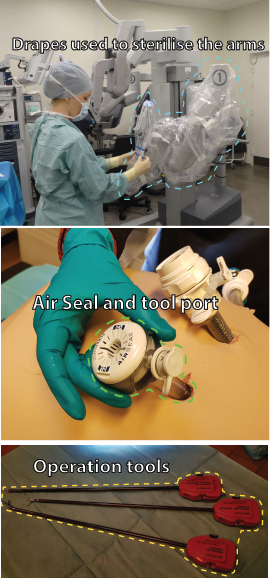
\includegraphics[width=0.48\textwidth]{Figures/fieldstudyresults.png}
\caption{Key objects during robot surgery. The robot arms of the da Vinci robot, ports used to insert the laparoscopic tools into the patient}
\label{Fig:fieldresult}
\end{figure}

\section{Methods}
This section provides information about the methods used in designing a system capable of simulating team training for nurses in virtual reality and how it was tested. 

\subsection{Design}
System design and minimum implementation criteria was set after a series of observations and interviews with Jane Petersson and Johan Poulsen was conducted. Active observations of robot surgery, surgeon training and team training for nurse assistants were needed to assess the implementation requirements whereas semi-structured interviews with experts provided inspiration and informed the design of the system. 
Figure \ref{Fig:fieldresult} shows the most important objects during robot assisted minimally invasive surgery. The top image shows a nurse preparing the robot arms by covering them in drapes to sterilize the equipment. An important aspect of this preparation is to place the arms correctly to avoid collisions during surgery. The middle image shows the ports that are inserted in the patient. The placement and rotation of these is of importance and is therefore also an object of interest. The bottom image shows the operating tools that are latched on to the robot arms and through the ports on the patient. These tools perform a wide variety of tasks depending on the type of tool such as cutting and grabbing tissue.  
The interviews with Jane Petersson focused primarily on the important aspects of team training for surgical nurses. These were communication between nurses, understanding your role in the operating room and the introduction to the da Vinci robot. During training, the instructor will spend time with the trainees getting to know the robot and show important steps such as placement of the arms, insertion of ports and instruments, controls of the robot, and teach the different error messages. The nurses will then have to use their knowledge and communicate with each other when they are operating on a live pig later. This way they gain hand-on experience with the robot and its functionalities according to Jane Petersson. She also mentioned that it is important that the instructor or someone with RAMIS experience is nearby as sporadic questions always arise. The communication is therefore not only nurse-to-nurse, but also a largely nurse-instructor.
During RAMIS there are usually three nurses present, one surgeon, and one anaesthetic nurse or doctor. The surgeon will sit at the surgeon console, controlling the arms of the robot while looking into a stereoscopic display. The three nurses all have different responsibilities. These are the sterile nurse and the surgeon assistant (sometimes first nurse assistant) who assist the the surgery by providing the right tools, monitoring the patient, and are the surgeon's "eyes outside of the patient". The third nurse, called the circulating nurse or \textit{floor nurse} is not sterile and can therefore go in and out of the operating room as needed and perform tasks that would otherwise unsterilize (this is a word Oliver) the other nurses. An overview of the OR, together with the roles of each member of staff is visualized in Figure \ref{fig:overview} 

\begin{figure}[H]
 \centering
 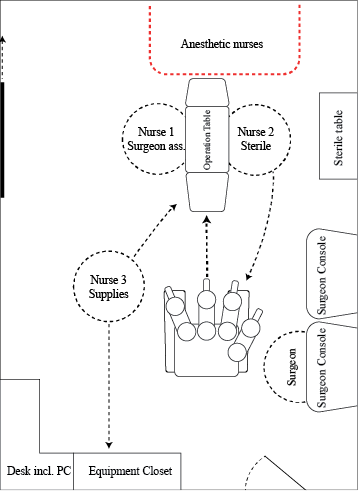
\includegraphics[width=0.48\textwidth]{Figures/overview.png}
 \caption{An overview of the operating room from the field observations}
 \label{fig:overview}
 \end{figure}
 
 The training room during team training is much smaller than the OR and space can be a problem in this context. Another benefit of virtualizing team training would therefore be more space.

Observations of the team training emphasized the importance of precision. When dealing with surgery every variable is situation dependent. This means there is no universal way of e.g. placement and orientation of the ports and tools, tilt of operating table, or even manual control of the laporascopic tools. These procedures require concentration and are constantly evaluated and corrected by the nurse performing them. Some of the primary feedback they get is from the screens placed in the room. These screens show the camera inside the patient and they use this to optimize their precision when working. 
Observations also led to the conclusion that a lot of questions arise during the training. These questions are often pointed at the instructor. The instructor then gives an in-depth answer while often also visualizing it using the tools and robot. These questions come sporadically and often unpredictably and it is therefore important that an instructor is nearby to make sure the procedure continues. Team training also prepare the nurses for emergencies, especially emergency undocking of the robot. When an emergency undocking is issued, the two nurses at the robot has to remove the arms and the ports on the patient and prepare for an open surgery, while the circulating nurse assists by calling for assistance and preparing the surgeon for open surgery. During this procedure precision and accuracy is not important, instead the time taken to perform the procedure becomes essential. 

Based on our field work .... 
We used Unreal engine to.... 

Interviews, observations, artefact models and all field work leading to the design of the robot, room and tasks implemented in the current system. Remember to argue for the lack of precision in the simulator and why we implemented emergency undocking since everything else in team training is not viable. 
Then instead we focus on the usability and make a shader that outline objects of interest, enable communication between participants, multiplayer, and in general make an exploratory project instead. We aim to answer if VR and Nurse team training is viable and what future projects should focus on when implementing in this context in VR. OUr experience is that there's a lot of talking and that's why it is necessary to have communication. There's a lot of showing and situation dependent illustrations that is not viable within our time constraints. 
Remember to mention that we designed it all in unreal engine 4 and with the htc vive headset. 
An idea in unrealæ was to implement IK hanldes and make the robot interactable but Unreal does not allow for this since the FABRIK affector position cannot be interacted with in real time. 
\subsection{Evaluation}

Two types of tests were performed, a usability test and an expert review with Jane Petersson and Johan Poulsen, head surgeon at AUH. Both tests were part of a system review. The system allowed multiple concurrent users to act in an operation environment with the intent of ultimately allowing RAMIS surgeons and nurses to train specific scenarios in VR with emphasis on communication and routine. The scenarios implemented in the test system are described in this section. The test procedure is listed below:

\begin{itemize}
\item Participants are introduced to the system and the project
\item The usability participants are split up in different rooms
\item The participants perform the required tasks together
\item Usability test participants fill out questionnaires
\item A short exit interview was held
\end{itemize}

The VR environment allowed participants to interact with a virtual robot modelled after the da Vinci Si, see Figure XX. They were able to move the arms and fit it with tools. Additionally, they were able to interact with items such as scrubs found in the room, which was modelled after the AUH robotic operating room, as shown in Figure XX. 

The scenario simulated was chosen based on interviews with Jane Petersson. It tasked participants with calibrating the robot arms by moving the tools to the "patient's" body. Afterwards, they were tasked with performing an emergency undocking together, going to open surgery. An overview of roles and tasks during emergency undocking is shown in Figure XX. This scenario was chosen since it enables training vital procedures that can be relatively accurately represented in VR. According to Jane Petersson, these are the most important tasks to train since they are what trainees undergoing team training at MIUC usually struggle the most with. Additionally, it would allow trainees to practice emergency procedures in a safe environment. Each participant was randomly assigned a role matching one shown in Figure XX, and informed of their tasks as the scenario progressed through a graphical user interface (GUI).

The participants used three HTC Vive head mounted displays (HMDs) connected to a server hosted on computer A. Computer C was located in a separate room from computer A and B. The specifications of these computers are shown in Table \ref{TAB:specs}. 

\begin{table}[H]
\centering
\begin{tabularx}{0.48\textwidth}{X X X X}
\toprule
                     & \textit{Computer A} & \textit{Computer B} & \textit{Computer C} \\ \midrule \rowcolor{lightGrey}
\textbf{CPU}         & Intel Core i7-6700K & Intel Core i7-4770  & x                   \\

\textbf{GPU}         & Nvidia GTX 1080     & Nvidia GTX 980      & Nvidia GTX 980Ti    \\  \rowcolor{lightGrey}

\textbf{Motherboard} & x                   & x                   & x                   \\ \toprule
\end{tabularx}
\caption{Specifications of the computers used}
\label{TAB:specs}
\end{table}

Prior to the test, participants were informed of the two actions they could perform, namely grabbing (using the HTC Vive controller's trigger) and teleporting (using the touchpad on the controller). Teleporting is important in VR since there is limited space to move around in the real world, and thus participants were also cautioned not to move outside the bounds shown in the world by poles. They were also informed about the possibility of VR sickness [cite XX] and that should it happen, they were to inform the observers and disengage from the system.

During the tests, participants were observed on the computers. They were able communicate in-room and through microphones located in the rooms. In the event of system error or when participants forgot tasks, controls, or otherwise were confused, facilitators were present to assist. 

After the test, participants were given a questionnaire. The questionnaires used in the usability test contain rating scales that rates different measures of the system complying to the System Usability Scale (SUS). These are shown in appendix XX. It also contained additional questions about the participants age, gender, familiarity with VR, and XX. Following that, a short interview was held to ensure their experience matched the expectations of the test, primarily to ensure they understood the tasks. Participant performance was not observed.

An expert review was held after the usability test to assess the utility of the system qualitatively. This review is also done to determine if there are critical errors in the simulation. Jane Petersson and Johan Poulsen both participated in this interview after observing and trying the system themselves. The review followed a simple structure with a facilitator and an observer. The results from this review were used to determine the viability of the system in context.
The script and transcript for the interview can be found in appendix XX.

%The scene used for testing is described in Section \ref{}. This scene was created to facilitate a simulated emergency undocking of the da Vinci robot. We used the contextual study to create the following procedure: REPEAT
  
\section{Results}
What did we find out

This is discussion

None of the participants in the usability test were trained in the medical field, which affects the validity of the results. This is an acceptable risk given that this is a usability test and not a utility focused test. 

\section{Conclusion}
What does it mean

% conference papers do not normally have an appendix


% use section* for acknowledgment
\section*{Acknowledgment}
The authors would like to thank Jane Petersson and Johan Poulsen at the MIUC department on Aalborg University Hospital for participation and engagement in the project. And for letting us observe training sessions as well as an operation.

% trigger a \newpage just before the given reference
% number - used to balance the columns on the last page
% adjust value as needed - may need to be readjusted if
% the document is modified later
%\IEEEtriggeratref{8}
% The "triggered" command can be changed if desired:
%\IEEEtriggercmd{\enlargethispage{-5in}}

% references section

% can use a bibliography generated by BibTeX as a .bbl file
% BibTeX documentation can be easily obtained at:
% http://mirror.ctan.org/biblio/bibtex/contrib/doc/
% The IEEEtran BibTeX style support page is at:
% http://www.michaelshell.org/tex/ieeetran/bibtex/
%\bibliographystyle{IEEEtran}
% argument is your BibTeX string definitions and bibliography database(s)
%\bibliography{IEEEabrv,../bib/paper}
%
% <OR> manually copy in the resultant .bbl file
% set second argument of \begin to the number of references
% (used to reserve space for the reference number labels box)
\begin{thebibliography}{1}

\bibitem{IEEEhowto:kopka}
H.~Kopka and P.~W. Daly, \emph{A Guide to \LaTeX}, 3rd~ed.\hskip 1em plus
  0.5em minus 0.4em\relax Harlow, England: Addison-Wesley, 1999.

\end{thebibliography}




% that's all folks
\end{document}


